\chapter{Benutzeranleitung}

\hypertarget{missionlist}{\section{Missionsliste}}

\begin{figure}[H]
	\centering
	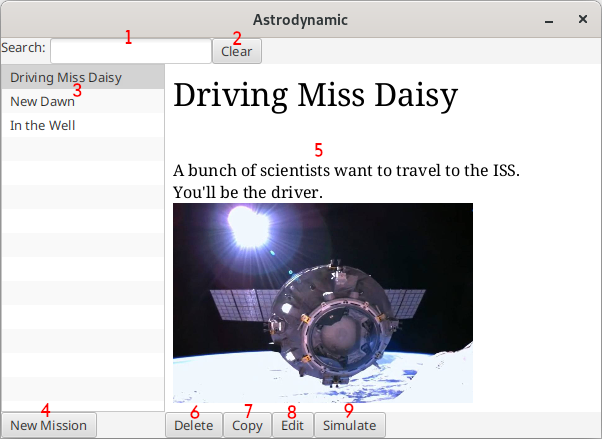
\includegraphics[width=12cm]{res/missionsliste.png}
	\caption{GUI Missionsliste mit Annotation}
\end{figure}

\begin{enumerate}[noitemsep]
	\item Suchfeld
	\item Clear: Suchfeld leeren
	\item Liste verfügbarer Missionen
	\item New Mission: Neue Mission öffnen im Missions-Editor
	\item Beschreibung der ausgewählten Mission
	\item Delete: Ausgewählte Mission löschen
	\item Copy: Ausgewählte Mission kopieren
	\item Edit: Ausgewählte Mission öffnen im Missions-Editor
	\item Simulate: Ausgewählte Mission öffnen im Simulator
\end{enumerate}

\subsection{Grundlagen}
Die Missionsliste ist der Einstiegsbildschirm beim Start des Programs.
Hat der Benutzer keine Mission gespeichert welche geladen werden kann so werden drei Testmissionen geladen.
Am linken Rand befindet sich die Liste der verfügbaren Missionen.Anwählen einer Mission in der Liste per Klick mit der Linken Maustaste lädt die Missionsbeschreibung in den rechten Anzeigebereich und ermöglicht mit diese Mission per Buttons unten rechts am Bildschirmrand weiter zu Interagieren.

\subsection{Missionen nach Beschreibung suchen}
Das Suchfeld führt eine sofortige Textsuche auf Missions-Name und -Beschreibung durch und zeigt auf Basis dieser nur passende Missionen in der Liste der verfügbaren Missionen. Durch drücken des Clear-Buttons können längere Sucheingaben sofort gelöscht und die Sortierung zurückgesetzt werden.

\begin{figure}[h]
	\centering
	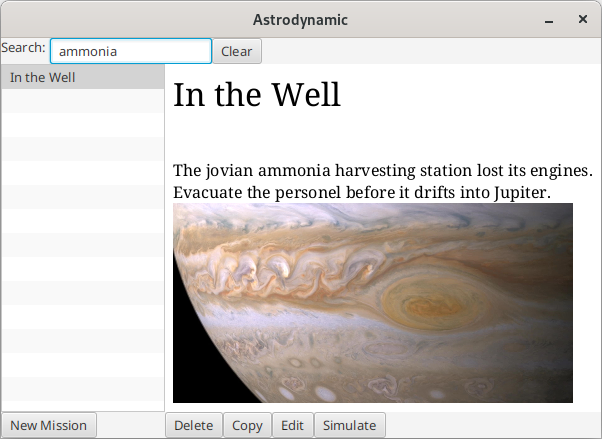
\includegraphics[width=8cm]{res/search.png}
	\caption{Missionsfilter bei Suche nach 'ammonia'}
\end{figure}

\subsection{Anlegen einer neuen Mission}
Klicken sie auf den ''Neue Mission öffnen im Missions-Editor''-Button unten links.
Es öffnet sich nun der Missions-Editor.
Für Details zum editieren einer Mission konsultieren sie das \hyperlink{missioneditor}{Kapitel Missions-Editor}.

\subsection{Löschen einer Mission}
Wählen sie die Mission aus der Liste der verfügbaren Missionen per Mausklick aus.
Klicken sie auf Delete.
Ein Popup öffnet sich mit der Löschanfrage.

\begin{figure}[H]
	\centering
	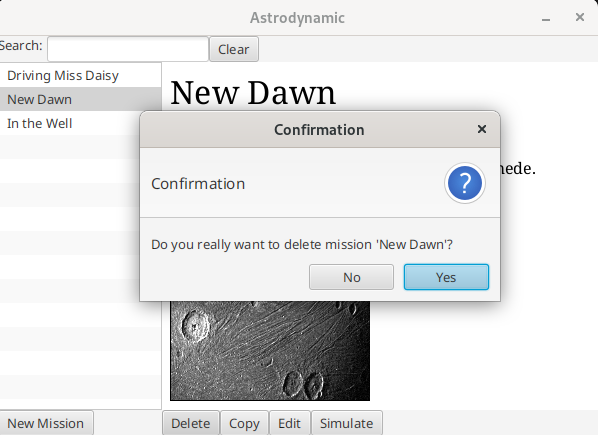
\includegraphics[width=8cm]{res/loeschen.png}
	\caption{Sicherheitsabfrage bei Missionslöschung}
\end{figure}

Bestätigen sie das Popup mit Klick auf Yes.
Die Mission wird aus der Liste der verfügbaren Missionen entfernt.

\subsection{Kopieren einer Mission}
\unimplemented
Wählen sie die Mission aus der Liste der verfügbaren Missionen per Mausklick aus.
Klicken sie auf Copy.
Es öffnet sich nun der Missions-Editor mit der kopierten Mission.
Für Details zum editieren einer Mission konsultieren sie das \hyperlink{missioneditor}{Kapitel Missions-Editor}.

\subsection{Editieren einer Mission}
Wählen sie die Mission aus der Liste der verfügbaren Missionen per Mausklick aus.
Klicken sie auf Edit.
Es öffnet sich nun der Missions-Editor mit der ausgewählten Mission.
Für Details zum editieren einer Mission konsultieren sie das \hyperlink{missioneditor}{Kapitel Missions-Editor}.

\subsection{Simulieren einer Mission}
Wählen sie die Mission aus der Liste der verfügbaren Missionen per Mausklick aus.
Klicken sie auf Simulate.
Es öffnet sich nun der Simulator mit der ausgewählten Mission.
Für Details zum simulieren einer Mission konsultieren sie das \hyperlink{simulator}{Kapitel Simulator}.

\hypertarget{missioneditor}{\section{Missions-Editor}}

\begin{figure}[H]
	\centering
	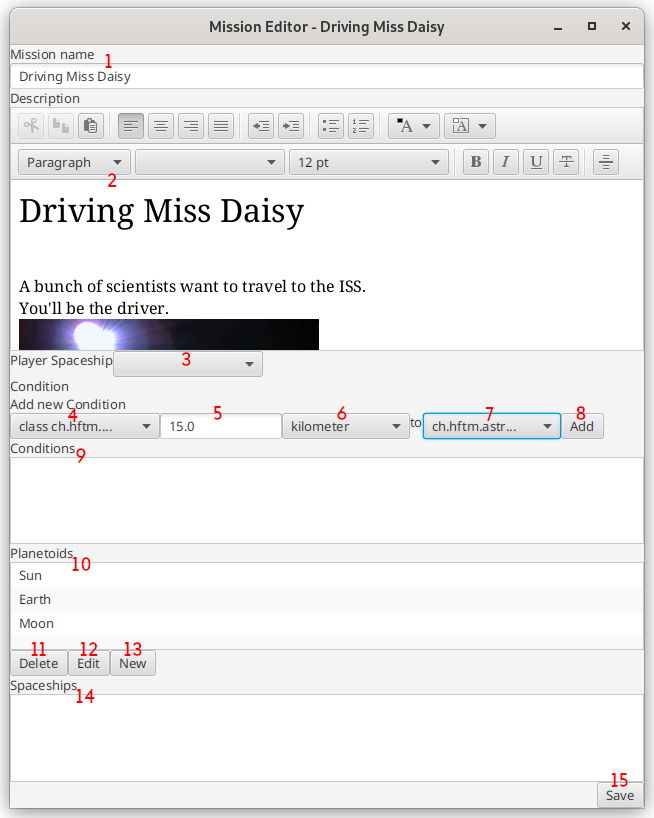
\includegraphics[width=12cm]{res/missioneditor.png}
	\caption{GUI Mission-Editor mit Annotation. Testmission 'Driving Miss Daisy' geöffnet.}
\end{figure}

\begin{enumerate}[noitemsep]
	\item Missionsname
	\item Missionsbeschreibung HTML-Editor
	\item Auswahl Spielerraumschiff
	\item Missionsbedingung: Bedingungstyp-Dropdown
	\item Missionsbedingung: Zahlenfeld
	\item Missionsbedingung: Masseinheit-Dropdown
	\item Missionsbedingung: Referenzobjekt-Dropdown
	\item Missionsbedingung hinzufügen
	\item Missionsbedingungen-Liste
	\item Planetoiden-Liste
	\item Planetoid entfernen
	\item Planetoid editieren
	\item Planetoid hinzufügen
	\item Raumschiff-Liste
	\item Missionsänderungen speichern
\end{enumerate}

\subsection{Grundlagen}
Der Missions-Editor erlaubt das Ändern des Missions-Namen und Beschreibung. Durch das Hinzufügen von Missionsbedingungen, auch Conditions genannt, können Abbruchsbedinungen für die Simulation festgelegt und weitere dynamische Veränderungen an der Mission vorgenommen werden. Verwendete Planetoiden und Raumschiffe werden in den ensprechenden Listen aufgelistet.

\hypertarget{addcondition}{\subsection{Hinzufügen einer Missionsbedingung}}
Wählen sie im Bedingungstyp-Dropdown den passenden Bedingungstypen.
Zahlenfeld, Grössenangabe und Referenzobjekt werden dynamisch ein- oder ausgeblendet.

% nifty way to make two figures side by side
\begin{figure}[H]
	\centering
	\begin{minipage}[b]{0.45\textwidth}
		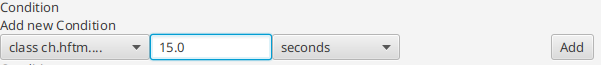
\includegraphics[width=\textwidth]{res/conditionmaxtime.png}
		\caption{MaximumTime}
	\end{minipage}
	\hfill
	\begin{minipage}[b]{0.45\textwidth}
		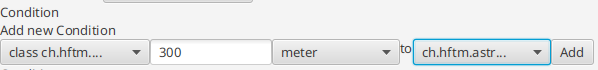
\includegraphics[width=\textwidth]{res/conditionapproach.png}
		\caption{Approach}
	\end{minipage}
\end{figure}

Sollte das Zahlenfeld oder das Referenzobjekt eingeblendet werden so ist eine Eingabe respektive Auswahl zwingend.
Die Masseinheit kann jederzeit geändert werden, ein valider Wert im Zahlenfeld wird in die neue Einheit umgewandelt.

\begin{figure}[H]
	\centering
	\begin{minipage}[b]{0.45\textwidth}
		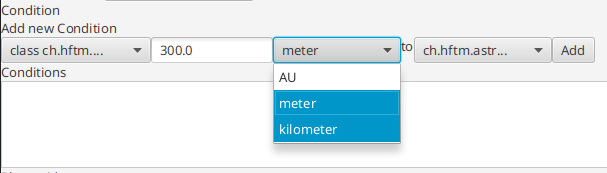
\includegraphics[width=\textwidth]{res/conditionunits.png}
		\caption{Masseinheit Meter}
	\end{minipage}
	\hfill
	\begin{minipage}[b]{0.45\textwidth}
		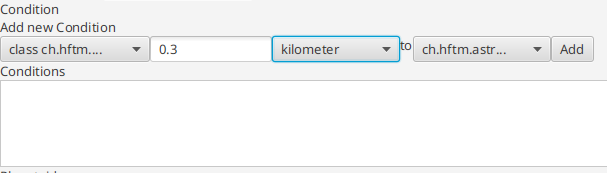
\includegraphics[width=\textwidth]{res/conditionunits2.png}
		\caption{Masseinheit Kilometer}
	\end{minipage}
\end{figure}

Klicken sie auf den Add-Button um die Missionsbedingung hinzuzufügen.
Die Missionsbedingung wird nun in der Missionsbedingungen-Liste aufgeführt.

\begin{figure}[H]
	\centering
	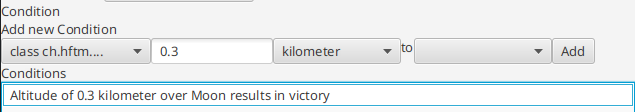
\includegraphics[width=0.45\textwidth]{res/conditionadded.png}
	\caption{Neue Approach-Missionsbedingung hinzugefügt}
\end{figure}

\subsection{Löschen eines Planetoiden}
Wählen sie den zu löschenden Planetoiden mit einem Klick aus der Planetoiden-Liste aus.
Klicken sie den Delete-Button.
Es öffnet sich eine Sicherheitsabfrage.

\begin{figure}[H]
	\centering
	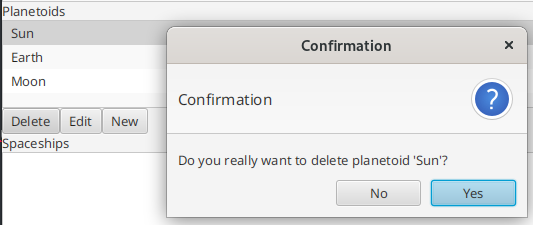
\includegraphics[width=0.45\textwidth]{res/loeschenplanetoid.png}
	\caption{Sicherheitsabfrage bei Planetoidenlöschung}
\end{figure}

Bestätigen sie das Popup mit Yes.
Der Planetoid ist nun aus der Mission entfernt und die Planetoiden-Liste aktualisiert worden.

\subsection{Editieren eines Planetoiden}
Wählen sie den zu editierenden Planetoiden mit einem Klick aus der Planetoiden-Liste aus.
Klicken sie auf den Edit-Button.
Es öffnet sich nun der Planetoid-Editior mit dem ausgewählten Planetoiden.
Für Details zum Planetoid-Editior konsultieren sie das \hyperlink{planetoideditor}{Kapitel Planetoid-Editior}.

\subsection{Hinzufügen eines Planetoiden}
\unimplemented

\subsection{Hinzufügen eines Raumschiffs}
Zum hinzufügen eines Raumschiffs benutzen sie die Condition 'SetupHeavyLander'.
Siehe \hyperlink{addcondition}{Abschnitt Hinzufügen einer Missionsbedingung}.

\hypertarget{planetoideditor}{\section{Planetoid-Editor}}

\hypertarget{simulator}{\section{Simulator}}